\documentclass[]{article}
\usepackage[utf8]{inputenc}
\usepackage[english]{babel}
\usepackage{polski}
\usepackage{fdsymbol}
\usepackage{amsfonts}
\usepackage{amsmath}
\usepackage{geometry}
\usepackage{fancyhdr} % do nagłówków
\usepackage{float} %precyzyjne umiejscowienie 
\usepackage{hyperref} %używanie hiperłączy
\usepackage{enumitem}
\usepackage{listings}
\usepackage[T1]{fontenc} %wymagane do używania zi4 (consolas podobne)
\usepackage{zi4}
\usepackage{color} %używanie kolorów
\usepackage[dvipsnames]{xcolor} %custom colory
\usepackage{graphicx} %do grafik
\newgeometry{tmargin=3.5cm}
\newgeometry{lmargin=2.5cm}
\newgeometry{bmargin=0.5cm}
\newgeometry{rmargin=2.5cm}
\definecolor{aqua}{RGB}{0 255 255} %nowy kolor
\definecolor{gray}{RGB}{49 54 59} %szary
\color{white} %domyślny kolor liter
\pagecolor{gray} %tło pliku
\setlength{\textheight}{23cm} %wysokość strony tekstu
\setlength{\topmargin}{-20mm} %domyślne ustawienie górnego marginesu na 1cal
\setlength{\parindent}{0mm} %usunięcie domyślnego wcięcia akapitu
\setcounter{section}{0} %numer pierwszej sekcji -1
\setcounter{page}{1}
\hypersetup{
	colorlinks=true, linkcolor=aqua, pdftitle=0 
}
\newcommand{\sspace}{\hspace*{3mm}}
\addto\captionspolish{\renewcommand{\contentsname}{\empty}}
\definecolor{codegreen}{RGB}{133, 153, 0}
\definecolor{codegray}{RGB}{147, 161, 161}
\definecolor{codepurple}{RGB}{ 108, 113, 196}
\definecolor{backcolour}{RGB}{ 7, 54, 66}

\lstdefinestyle{onestyle}{
	backgroundcolor=\color{backcolour},   
	commentstyle=\color{codegreen},
	keywordstyle=\color{magenta},
	numberstyle=\tiny\color{codegray},
	stringstyle=\color{codepurple},
	basicstyle=\ttfamily\scriptsize,
	breakatwhitespace=false,         
	breaklines=true,                 
	captionpos=b,                    
	keepspaces=true,                 
	numbers=left,                    
	numbersep=5pt,                  
	showspaces=false,                
	showstringspaces=false,
	showtabs=false,                  
	tabsize=2
}
\lstset{style=onestyle}

\title{WS281x}
\author{Author: Maciej Zbrzezny}
\date{}
\begin{document}
	\maketitle
	\pagestyle{fancy}
	\lhead{}
	\chead{}
	\rhead{Author: Maciej Zbrzezny}	
	\lfoot{}
	%\cfoot{\thepage}
	\section*{Table of contents}
	\cfoot{\hyperlink{}{\thepage}}
	\tableofcontents
	\newpage
	\section{How to use}
	\subsection{Required .ioc configuration (timer)}
	Make sure you have these set in your .ioc file:
	\begin{itemize}
		\item In project manager tick \textit{Generate peripheral initialization as pair of '.c/.h' files per peripheral}
		\item Choose timer and channel which can use DMA
		\item Timer must be in mode \textit{PWM Generation CHx} where x is number of chosen channel
		\item Set frequency to 800kHz (1.25 $\mu$s period) on your timer using \textit{Counter Period}. It's not recommended to have prescaler active.
		\item Add DMA request in DMA settings, choose direction to \textit{Memory to Peripheral}, make sure data width is \textit{Half Word} in Peripheral and Memory. Mode should be \textit{Normal} 
		\item if you use inverting logic level shifter, switch \textit{CH Polarity} to Low
	\end{itemize}
	\begin{minipage}{0.5\textwidth}
		\begin{figure}[H]
			\centering
			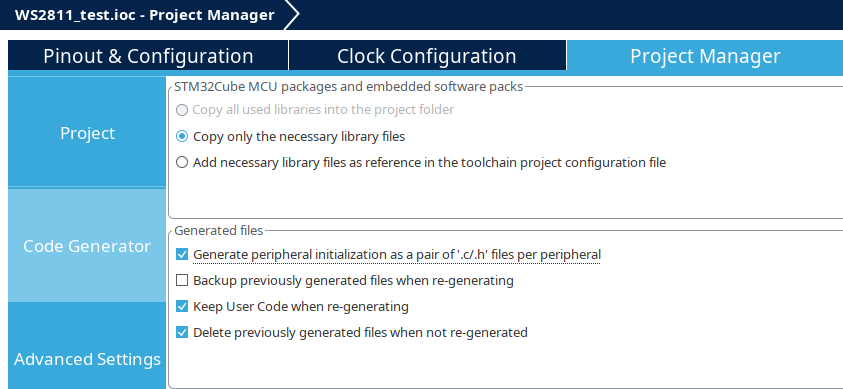
\includegraphics[width=0.9\linewidth]{separatedfiles}
			\caption{How to generate separated files}
			\label{fig:separatedfiles}
		\end{figure}
				
	\end{minipage}
	\begin{minipage}{0.5\textwidth}
		\begin{figure}[H]
			\centering
			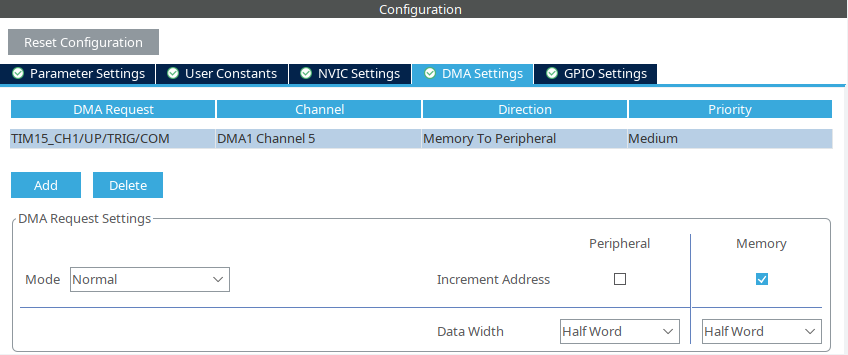
\includegraphics[width=0.9\linewidth]{dma}
			\caption{Sample DMA configuration}
			\label{fig:dma}
		\end{figure}		
	\end{minipage}
	\subsection{Required .ioc configuration (SPI)}
	\begin{minipage}{0.5\textwidth}
	Make sure you have these set in your .ioc file:	
	\begin{itemize}
		\item In project manager tick \textit{Generate peripheral initialization as pair of '.c/.h' files per peripheral}
		\item Choose your SPI and then mode: \textit{Half-Duplex Master}
		\item Set \textit{Data Size} to 6 Bits (if not possible then set 8 Bits), MSB First
		\item Set your \textit{Prescaler} to value which gives \textit{6-7MBits/s Baud Rate}, you may need to switch clock configuration
	\end{itemize}	
	\end{minipage}
	\begin{minipage}{0.5\textwidth}
		\begin{figure}[H]
			\centering
			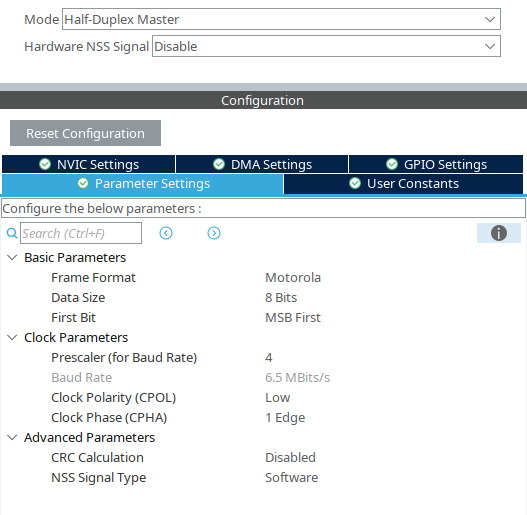
\includegraphics[width=0.8\linewidth]{SPI_config}
			\caption{SPI configuration}
			\label{fig:spiconfig}
		\end{figure}
	\end{minipage}	
	\subsection{Adding library}
	Just follow these steps:
	\begin{enumerate}
		 \item In command line (can be git bash or linux terminal) type:\\
			\begin{lstlisting}[language=bash]
git init
git submodule add https://github.com/MaciejZb66/ws281x.git
\end{lstlisting}
		\item Refresh project by clicking F5
		\item Add library path to build
		\begin{enumerate}[label*=\arabic*.]
			\item Left click on project and choose properties
			\item On left side choose \textit{C/C++ General}, then \textit{Paths and Symbols} and \textit{includes}
			\item Click on add button and find folder \textbf{ws281x}
			\item In \textit{Source Location} (still \textit{C/C++ General} and \textit{Paths and Symbols}) add folder \textbf{ws281x}
		\end{enumerate}
		\item In file \textit{main.h} add this line:\\
			\begin{lstlisting}[language=C]
#include "led.h"
\end{lstlisting}
	\end{enumerate}
			
	\begin{minipage}{0.5\textwidth}
		\begin{figure}[H]
			\centering
			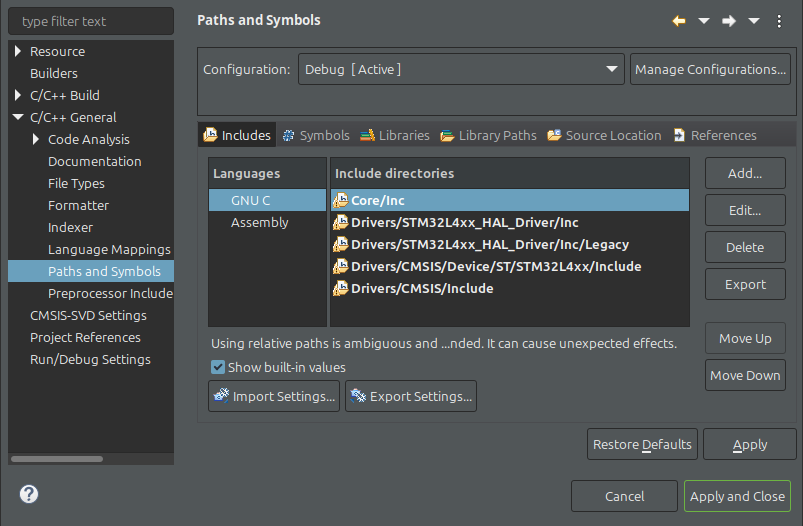
\includegraphics[width=0.9\linewidth]{Properties1}
			\caption{Add path to folder in includes}
			\label{fig:properties1}
		\end{figure}			
	\end{minipage}
	\begin{minipage}{0.5\textwidth}
		\begin{figure}[H]
			\centering
			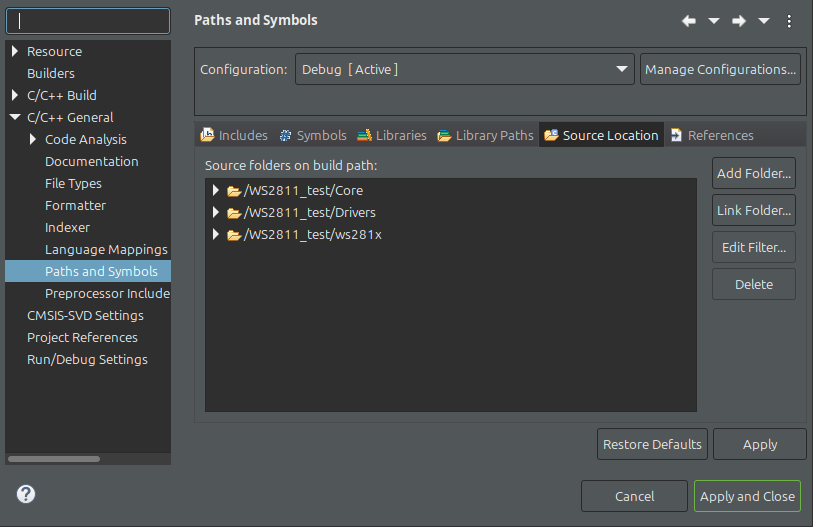
\includegraphics[width=0.9\linewidth]{Properties2}
			\caption{Add to source location}
			\label{fig:properties2}
		\end{figure}		
	\end{minipage}
	\subsection{Configuration file}
	This library is default configured in \textit{sample\_config.h} where we have:
				\begin{lstlisting}[language=C]
#define STM_FAMILY_L4
#define WS_TIM_15
#define WS_CHANNEL_1
#define user_leds 24
\end{lstlisting}
To redefine configuration create your own configuration file. There must be defined:
\begin{itemize}
	\item using timer or SPI (can be both)
	\item STM family
	\item number of outputs
	\item maximum number of LEDs (WS drivers connected to LEDs)
	\item \begin{lstlisting}[language=C]
#define WS_CONFIG //required to exclude sample_config.h \end{lstlisting}
	
\end{itemize} 
\subsection{Initialization}
To initialize your chosen timer use function:
\begin{lstlisting}[language=C]
void WS281x_init_TIM(WS281x_data* led, TIM_HandleTypeDef* htim, uint32_t t_channel, uint16_t led_number	\end{lstlisting}
To initialize your chosen SPI use function:
\begin{lstlisting}[language=C]
void WS281x_init_SPI(WS281x_data* led, SPI_HandleTypeDef* hspi, uint16_t led_number)	\end{lstlisting}
and give all required info. \texttt{WS281x\_data} is named LED and it's created as you define number of outputs. In both cases it's required to initialize once per output.
	\section{Code description}
	to be described later	
\end{document}
